\chapter{Introducción}


	Los microbolomeetros son bonitos y \cite{Hernandez2021}
	
	Porque los sistemas de adquisión de datos son tan importantes en la ciencia
	Cuales son las dificultades de realizar uno (depende de las especificaciones, el tiempo y el capital humano)
	Historia de los sistemas de adquisión de datos
	Ejemplos de sistemas de adquisión de datos
	Aplicaciones de sistemas de adquisión de datos
	Puedes enfocarlo al microbolometro o en general
    
    \section{Radiación Electromagnética}
    La radiación electromagnética es la emisión y transmisión de energía en forma de ondas electromagnéticas. El espectro electromagnético es una representación de los diversos tipos de radiación existentes, en él se definen los intervalos de longitudes de onda o frecuencia que cada una de ellas abarca \cite{Chang}.
            \begin{figure}[hbtp]
                \centering
                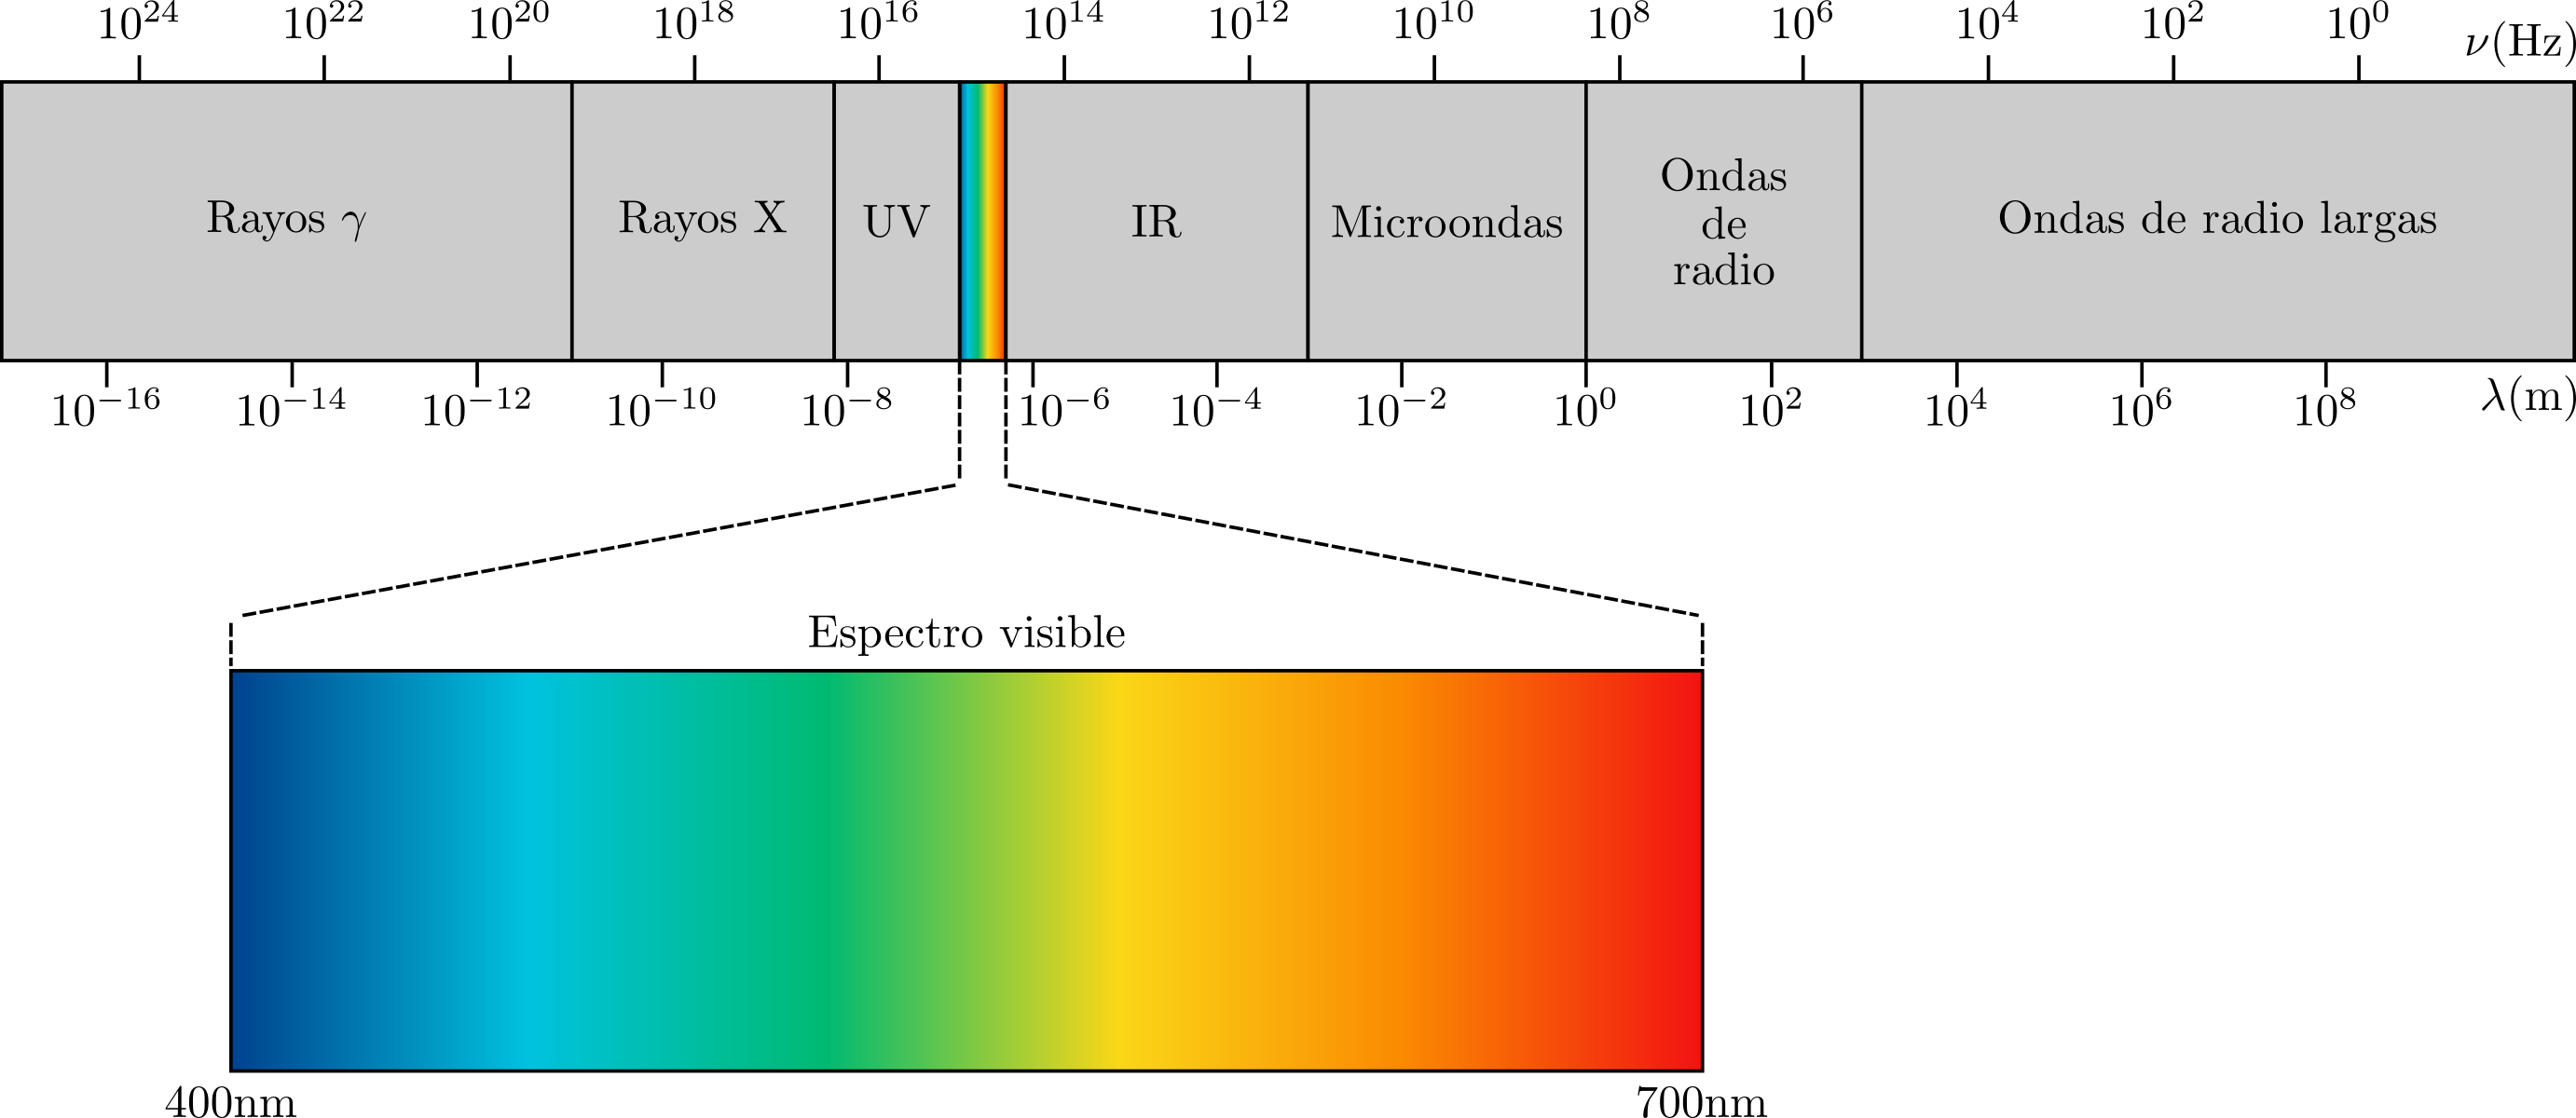
\includegraphics[width=0.8\textwidth]{espectro}
                \caption{Espectro electromagnético.}
                \label{fig:espectro}
            \end{figure}    
    
    Estas radiaciones obedecen las mismas leyes, la diferencia entre ellas radica en su longitud de onda o frecuencia, así como en la manera en que interactúan con los materiales ópticos, incluída la atmósfera \cite{Vincent}.
    
    Todos los cuerpos emiten radiación e.m  y debido al movimiento de sus átomos y moléculas se genera una temperatura en ellos. Los cuerpos con una temperatura mayor a 0K emiten radiación térmica por medio de ondas e.m. La radiación térmica es la radiación que emite un cuerpo por su temperatura \cite{Hollands}.\\
    La capacidad que tiene un cuerpo para emitir radiación está fuertemente relacionada con su capacidad de absorberla \cite{Beiser}.\\
    Una superficie ideal que absorbe toda la radiación que incide sobre él se denomina \textit{cuerpo negro} y el espectro de radiación que emite se llama \textit{radiación de cuerpo negro} \cite{Sears}.\\
    A pesar de que en la naturaleza no existe un objeto físico que pueda absorber toda la radiación incidente \cite{FUV3}, este puede representarse como un objeto hueco con una pequeña apertura donde cualquier radiación que incida en ella ingresa a la cavidad donde queda atrapada hasta que es absorbida \cite{Beiser}, \cite{FUV3}. En equilibrio térmico la radiación emitida por el cuerpo será exactamente igual a la absorbida.\\
    El cuerpo negro fue creado como una herramienta auxiliar para entender como los objetos emiten y absorben radiación.
    Hacia finales del siglo XIX la radiación de cuerpo negro ya había sido estudiada y dos leyes importantes sintetizaron los descubrimientos experimentales sobre este tema: La \textit{Ley de Stefan-Boltzmann} y la \textit{Ley de desplazamiento de Wien} \cite{FUV3}.\\
    
    La \textit{Ley de Stefan-Boltzmann} plantea que la intensidad de la radiación emitida por un cuerpo negro depende de su temperatura. La intensidad es proporcional a la cuarta potencia de la temperatura absoluta del cuerpo:
    
    \begin{equation}
        I = \sigma T^{4}
        \label{eq:Stefan-Boltzmann}
    \end{equation}
    
    Donde:\\
    $T$ es la temperatura del cuerpo negro en K.\\
    $\sigma$ es la constante de Stefan-Boltzmann, $\sigma = 5.670\times10^{-8}\ W/m^{2}K^{4}$\\
    
    La intensidad de la radiación no se distribuye uniformemente a lo largo de todas las longitudes de onda. En cambio, su distribución puede medirse y describirse utilizando la intensidad por intervalo de longitud de onda, $I(\lambda)d\lambda$.
            \begin{figure}[hbtp]
                \centering
                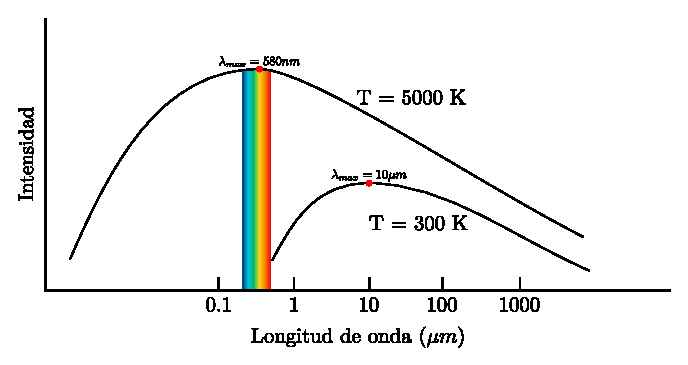
\includegraphics[width=0.8\textwidth]{intensidad_bb}
                \caption{Emitancia espectral de un cuerpo negro.}
                \label{fig:intensidad_bb}
            \end{figure}    
    \newpage
    La Figura \ref{fig:intensidad_bb} muestra las intensidades registradas a dos temperaturas diferentes. En cada caso hay una longitud de onda específica $\lambda_{m}$ en la que la intensidad de la radiación emitida es máxima.
    
    La \textit{Ley de desplazamiento de Wien} indica que cuando la temperatura de un cuerpo negro aumenta, la longitud de onda en la que se emite la radiación máxima se desplaza hacia valores más cortos:\\
    \begin{equation}
        \lambda_{m} = \frac{2.90\times10^{-3}\ mK}{T}
        \label{eq:Wien}
    \end{equation}  
    
    Donde:\\
    $\lambda_{m}$ es la longitud de onda en la que un cuerpo negro emite la mayor cantidad de radiación a una determinada temperatura \cite{Sears},\cite{FUV3}.\\
    
    De las leyes anteriores y la Figura \ref{fig:intensidad_bb} se puede deducir que la radiación UV, los rayos X y Gamma, son radiaciones más cálidas (radiaciones de alta energía), mientras que la radiación infrarroja está asociada a fenómenos con temperaturas cercanas a la temperatura ambiente \cite{Chang}, \cite{BlancoMDA}.     
    
    \section{Radiación Infrarroja} 
    La radiación infrarroja es un tipo de radiación electromagnética que cuenta con longitudes de onda mayores que las del rango visible. Se encuentra en el rango de 0.77$\mu m$ - 1$mm$ \cite{BlancoMDA}, y a su vez se divide en varias regiones las cuales se muestran en la Tabla \ref{tab:Div_IR}.
    
            \begin{table}[htbp]
                \caption{División de la radiación infrarroja\cite{Rogalski}}
                \begin{center}
                    \resizebox{0.8\linewidth}{!}{ 
                    \begin{NiceTabular}{ l c }
                        \CodeBefore
                        \Body
                        \textbf{Region}  & \textbf{Rango de frecuencia ($\mu m$)}\\
                        Near infrared (NIR)   & 0.78 - 1\\
                        Short wavelength IR (SWIR)   & 1 - 3\\
                        Medium wavelength IR (MWIR) & 3 - 6\\
                        Long wavelength IR (LWIR)  & 6 - 15\\
                        Very long wavelength IR (VLWIR) & 15 - 30\\
                        Far infrared (FIR)  & 30 - 100\\
                        Submillimeter (SubMM) & 100 - 1000
                    \end{NiceTabular}
                    }
                \label{tab:Div_IR}
                \end{center}
            \end{table}
            
            \newpage
            
Algunas de las aplicaciones de la radiación infrarroja son:
			\begin{itemize}
				\item \textbf{Visión nocturna}: Las cámaras de visión nocturna trabajan en el espectro infrarrojo para permitir la visión en la oscuridad, estas capturan la radiación térmica emitida por objetos y seres vivos.
				\item \textbf{Medicina}: Es utilizada para hallar cáncer y diabetes en el cuerpo humano.
				\item \textbf{Industria}: Inspección del estado de equipos eléctricos y mecánicos.
				\item \textbf{Conservación de energía}: Con escáneres IR se detectan pérdidas y fugas de calor en casas o industrias.
				\item \textbf{Ambientales}: Medición de la concentración de diversos gases contaminantes en la atmósfera.
				\item \textbf{Agricultura}: Monitoreo del estado de los cultivos y la salud de las plantas, la humedad del suelo y la presencia de plagas o enfermedades.
				\item \textbf{Astronomía}: Los telescopios infrarrojos permiten estudiar regiones del espacio donde se están formando estrellas.
				\item \textbf{Espectroscopía}: Usada en química y biología para identificar y analizar estructuras moleculares de sustancias.		
			\end{itemize}
\cite{Rogalski}, \cite{BlancoMDA}.

La mayoría de las aplicaciones en detección de radiación infrarroja requieren que esta se transmita a través del aire \cite{Jimenez}. La atmósfera terrestre se compone de ozono ($O_{3}$), dióxido de carbono ($CO_{2}$) y vapor de agua ($H_{2}O$). Estas moléculas bloquean algunas regiones del espectro infrarrojo, impidiendo la transmisión de la radiación IR a la atmósfera. Las longitudes de onda que no son afectadas por estas moléculas reciben el nombre de ventanas atmosféricas \cite{Rogalski}, \cite{Motilal}. En la Figura \ref{fig:atmos_window} podemos observarlas.\\

            \begin{figure}[hbtp]
                \centering
                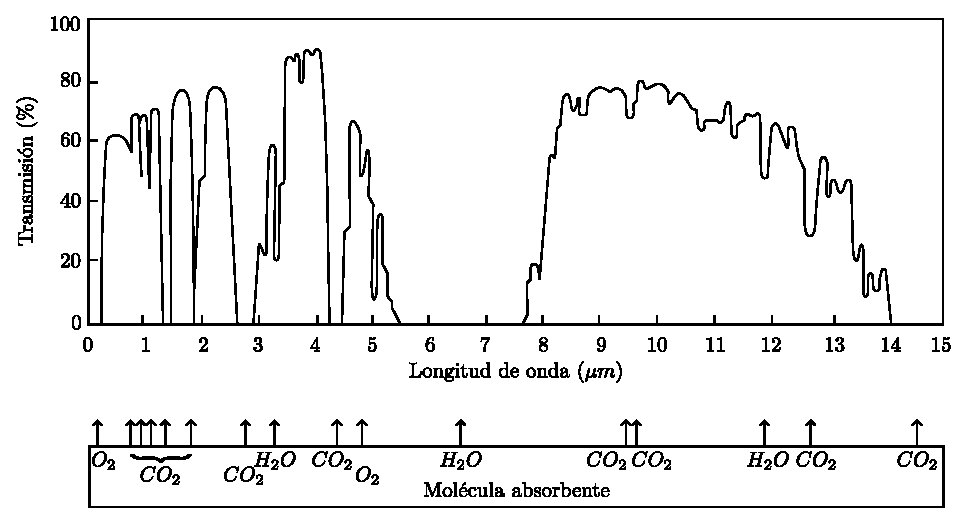
\includegraphics[width=0.8\textwidth]{atmos_window}
                \caption{Transmisión de la atmósfera.}
                \label{fig:atmos_window}
            \end{figure}



Despejando la temperatura de la \textit{Ley de desplazamiento de Wien} (ecuación \ref{eq:Wien}) \cite{BlancoMDA}:
    \begin{equation}
        T_{max} = \frac{2.90\times10^{-3}\ mK}{8\mu m} = 362.5K
        \label{eq:tempmax}
    \end{equation}

    \begin{equation}
        T_{min} = \frac{2.90\times10^{-3}\ mK}{14\mu m} = 207.14K
        \label{eq:tempmin}
    \end{equation}

podemos deducir que los detectores infrarrojos que operan en la ventana de 8 - 14 $\mu m$ tienen mayor sensibilidad a la temperatura ambiente \cite{Rogalski}.\\

El material de fabricación y longitud de onda de operación de los detectores infrarrojos cambian de acuerdo a la aplicación en la que se desee trabajar \cite{Rogalski}.					           
     
    
    \section{Detectores Infrarrojos}
    
    Un detector infrarrojo es un dispositivo capaz de absorber parte de la energía infrarroja radiada hacia él, provocando una variación en alguna de sus propiedades eléctricas \cite{BlancoMDA}. Podemos pensar en un detector infrarrojo como un transductor, el cual convierte un tipo de señal en otra; el detector infrarrojo convierte la radiación infrarroja incidente en una señal eléctrica \cite{Vincent}.
    
    Dependiendo de la aplicación, el rango del espectro electromagnético y la temperatura en los que se desee trabajar, se debe diseñar o utilizar un detector específico que cumpla con los requerimientos, ya que cada aplicación requiere características diferentes a las demás \cite{BlancoMDA}, \cite{Rogalski}.\\
    Los detectores infrarrojos se pueden clasificar en dos categorías: \textit{Detectores de fotones} y \textit{detectores térmicos}.
    
		\subsection{Detectores de fotones} 
		   
		\subsection{Detectores térmicos}
		
		\begin{enumerate}
		    \item Resistivos
		\end{enumerate}
		 
				          
		
    \section{Objetivos}
	
		\subsection{Objetivo general}
			\begin{itemize}
				\item Diseño de un sistema de adquisición de datos basado en FPGA para la medición de una matriz de pixeles de un microbolómetro.
			\end{itemize}
		
		\subsection{Objetivos específicos}
			\begin{itemize}
                \item Obtención de especificaciones para el sistema de adquisición de datos.
                \item Selección de ADC y DAC y protocolo de comunicación a partir de las especificaciones.
                \item Diseño de un firmware en el lenguaje de descripción de hardware (HDL) Verilog para el protocolo de comunicación SPI reconfigurable y robusto.
                \item Implementación de protocolo SPI para control de un ADC y un DAC de 12 bits.
                \item Pruebas experimentales y de estrés para verificación de robustes del diseño y mejora.
                \item Adquisición de los datos utilizando una terminal de usuario basada en UART.
			\end{itemize}
